\PassOptionsToPackage{usenames,dvipsnames}{xcolor}
\documentclass[twocolumn,twocolappendix]{aastex63}

% Add your own macros here:
\pdfoutput=1 %for arXiv submission
%\usepackage{amsmath,amssymb,amstext}
\usepackage{amsmath,amstext}
\usepackage[T1]{fontenc}
\usepackage{apjfonts}
\usepackage{ae,aecompl}
\usepackage[utf8]{inputenc}
\usepackage[figure,figure*]{hypcap}

\usepackage{url}
\urlstyle{same}

\usepackage{lineno}
\linenumbers
%\modulolinenumbers[2]

\newcommand{\placeholder}[1]{\textit{PLACEHOLDER: #1}}

\newcommand{\EiffL}[1]{{\color{cyan}FL: #1}}


% header settings
\shorttitle{Differentiable Lensing Simulations}
\shortauthors{Lanzieri et al.\ (LSST~DESC)}

% ======================================================================

\begin{document}
\title{Forecasting the power of Higher Order Weak Lensing Statistics with automatically differentiable simulations}
\collaboration{1000}{The LSST Dark Energy Science Collaboration (LSST DESC)}
\noaffiliation

% paper leads
\author{Denise Lanzieri}
\affiliation{Université Paris Cité, Université Paris-Saclay, CEA, CNRS, AIM, F-91191, Gif-sur-Yvette, France}

\author[0000-0001-7956-0542]{Fran\c{c}ois Lanusse}
\affiliation{Université Paris-Saclay, Université Paris Cité, CEA, CNRS, AIM, 91191, Gif-sur-Yvette, France; }

%First Tier authors (alphabetical)
\author{Chirag Modi}
\affiliation{Center for Computational Astrophysics,
Center for Computational Mathematics,
Flatiron Institute, New York, NY 10010, USA}
% \noaffiliation

\author{Benjamin Horowitz}
\affiliation{Lawrence Berkeley National Laboratory, 1 Cyclotron Road, Berkeley, 94720, CA, USA}
\affiliation{Department of Astrophysical Sciences, Princeton University, Princeton, NJ 08544, USA}


\author{Joachim Harnois-Déraps}
\affiliation{School of Mathematics, Statistics and Physics, Newcastle University, Herschel Building, NE1 7RU Newcastle-upon-Tyne, UK}
% Second Tier authors (alphabetical)
\author{Jean-Luc Starck}
\affiliation{Université Paris-Saclay, Université Paris Cité, CEA, CNRS, AIM, 91191, Gif-sur-Yvette, France; }

\begin{abstract}
In this project we investigate the relative constraining power of various map-based higher order weak lensing statistics in an LSST setting. Such comparisons are typically very costly as they require a large number of simulations, and become intractable for more than 3 or 4 cosmological parameters. Instead we propose a new methodology based on the TensorFlow framework for automatic differentiation, and more specifically the public FlowPM N-body simulation code. By implementing ray-tracing in this framework, we will be able to simulate lensing lightcones, and compute Higher Order lensing statistics on the resulting maps. These statistics can then be differentiated with respect to cosmology, or any systematics included in the simulations, thus allowing, for exact Fisher forecasts.
\end{abstract}

\keywords{methods: statistical -- dark energy}

%\accepted{}
%\submitjournal{the Astrophysical Journal Supplement}


%\tableofcontents%-----------------------------
%===========================
% BEGINNING OF THE MAIN TEXT
%===========================

\section{Introduction}

\section{FlowPM}

\section{Ray-tracing}
In this section, we provide a brief overview of the lensing convergence and the basic concepts of cosmic shear.
Weak gravitational lensing is a promising observational technique to infer the projected matter density distribution between an observer and a source by measuring galaxy shape correlations. 

In a homogeneous FLRW Universe, the geodesic equation of Light ray trajectories induced by the density fluctuations are expressed as :
\begin{equation}\label{geod}
    \frac{d^2\textbf{x}_{\bot}(\chi)}{d\chi^2}
    = -2 \nabla_{\bot} \Phi(\textbf{x}_{\bot},\chi).
\end{equation}
If we integrate Eq.\ref{geod} over the line of sight along $\chi'$ the solution $\textbf{x}_{\bot}$ for the radial comoving distance becomes:
\begin{equation}
    \textbf{x}(\chi)=f_k(\chi)\boldsymbol{\theta}-\frac{2}{c^2} 
    \int_0^{\chi} d\chi'f_k(\chi-\chi')[\boldsymbol{\nabla}_{\bot}\Phi(\textbf{x},\chi')-\boldsymbol{\nabla}_{\bot}\Phi^{(0)}(\chi')]
\end{equation}
 where we indicate as $f_k(\chi)$ and $\chi$ the angular and radial comoving distance, respectively.
 In the absence of lensing the observer would see the distance \textbf{x} under an angle $\boldsymbol{\beta}$$=\textbf{x}(\chi)/f_k(\chi)$.
 
 In the presence of lensing the separation vector \textbf{x} will be seen under an angle $\boldsymbol{\alpha}$, defining as:
 \begin{equation}
     \boldsymbol{\alpha}=\frac{2}{c^2} \int_0^{\chi} d\chi'
     \frac{f_k(\chi-\chi')}{f_k(\chi)}
     [\boldsymbol{\nabla}_{\bot}\Phi(\textbf{x},\chi')-\boldsymbol{\nabla}_{\bot}\Phi^{(0)}(\chi')].
 \end{equation}
 So that, the difference between the apparent angle $\theta$ and the source position $\beta$ defines the lens equation:
 \begin{equation}
 \boldsymbol{\alpha=\theta - \beta}.
 \end{equation}
In the next section we will infer the lensing potential  $\Phi$ by solving the Poisson equation from the three dimensional density contrast $\delta$:
\begin{equation}\label{Poisson}
    \nabla_{\bot}^2 \Phi(x_{\bot},\chi)=
    \frac{3H_0^2 \Omega_m}{2c^2a(\chi)}
    \delta(x_{\bot},\chi)
\end{equation}
where we indicate as $a$ the scale factor, and  as $\Omega_m$ and $H_0$ the matter density and the Hubble parameter, respectively. 

\subsection{The Born approximation}

We know that the knowledge of the lensing potential and the use of accurate solvers for light ray trajectories could be computationally expensive.
For this reason, in this work we implement the Born approximation, integrating the potential gradient along the unperturbed ray. If we consider the series expansion in powers of $\Phi$, assuming that the $\Phi$ is small and considering just the first-order approximation, the gravitational potential  can be written as:
\begin{equation}
    \Phi(f_k(\chi')\boldsymbol{\theta},\chi').
\end{equation}
We can now define the Jacobian matrix \textbf{A}$=\partial\boldsymbol{\beta}/\partial\boldsymbol{\theta}$, describing the linear mapping from the lensed image to the unlensed source:
\begin{align}
    A_{ij}=& \frac{\partial\beta_i}{\partial\theta_j}=
    \delta_{ij}-\frac{\partial\alpha_i}{\partial\theta_j} \\
     & =\delta_{ij}-\frac{2}{c^2}
    \int_0^{\chi} d\chi'
     \frac{f_k(\chi-\chi')f_k(\chi')}{f_k(\chi)}
     \frac{\partial^2}{\partial x_i \partial x_j} \Phi(f_k(\chi')\boldsymbol{\theta},\chi').
\end{align}
From the parametrization of the symmetrical matrix \textbf{A}, we can define the spin-two shear $\gamma=(\gamma_1,\gamma_2)$ and the scalar convergence field, $\kappa$. 
Considering this definition the convergence and the shear are defined as second derivative of the potential:
\begin{equation}\label{kshear}
    \kappa=\frac{1}{2}(\partial_1\partial_1+\partial_2\partial_2)\psi; \ \gamma_1=\frac{1}{2}(\partial_1\partial_1-\partial_2\partial_2)\psi; \ 
    \gamma_2=\partial_1\partial_2\psi;
\end{equation}
where we define the 2D \textit{lensing potential} $\psi$,
\begin{equation}
    \psi(\boldsymbol{\theta},\chi)=
    -\frac{2}{c^2}
    \int_0^{\chi} d\chi'
     \frac{f_k(\chi-\chi')f_k(\chi')}{f_k(\chi)}
    \Phi(f_k(\chi')\boldsymbol{\theta},\chi').
\end{equation}
The two fields $\gamma$ and $\kappa$ describe the distortion in the shape of the image, and the change in the angular size, respectively.
Considering the Eq.\ref{Poisson} and the Eq.\ref{kshear} the convergence $\kappa$ becomes:
\begin{equation}
    \kappa_{born}(\boldsymbol{\theta},\chi_s)= \frac{3H_0^2 \Omega_m}{2c^2}
    \int_0^{\chi_s} 
    \frac{d\chi'}{a(\chi')}
     \frac{f_k(\chi-\chi')}{f_k(\chi)}
     f_k(\chi')
    \delta(f_k(\chi')\boldsymbol{\theta},\chi').
\end{equation}

%\begin{equation}
%where $n(\chi)$ is a redshift independent factor of normalization from Poisson equation.
 %   n(\chi)=(AB)(\chi^2)
%\end{equation}
%where $A$ is the two dimensional mesh area in $rad^2$ per pixel and $B$ is the mean 3 dimensional particle density in the all cube.


\section{Methods}

Our weak lensing simulation tool is based on FlowPM (/cite Modi, Lanusse et al. ), a fast particle-mesh solver that implements the time integration for gravitational evolution starting from the Gaussian initial conditions of the Universe to the observed large scale structures through a Kick-Drift scheme.


After instantiating the $\Lambda$CDM cosmology with our desired parameters, (the initial power spectrum and the evolution of the particles depend from $\sigma_8$ and $\Omega_{c}$) we created the initial condition for the N-body simulation using the normalised linear matter power spectrum as implemented by (/cite Eisenstein and Hu of '98 ) and generated the linear field at requested scale. After that, we implemented the N-body. As said before, The N-body simulation does the time integration of a given initial linear field  across a given array of scale factors implementing a series of Kick-Drift-Kick operations. 
During the \textit{Kick} operation we estimate the gravitational force experienced by every particles implementing Fast Fourier Transform and update their momentum. In the next state, \textit{Drift}, the particles are displaced and their positions is updated with the velocity estimated in the previous step. This operation is continued until the observed large scale structures at the final time-step.
To perform the lightcone computation and extract the lens planes,  we export several intermediate state from the N-body simulation. From a given intermediate state we extract a slice and project it as a density plane by painting the particles on a 2D mesh. 
After creating a grid of coordinates, the lens planes are interpolated onto sky coordinates. 
 At this point, we have constructed a ray tracer object, to compute the convergence, we directly integrate the lensing density along the unperturbed line of sight. 

    
\section{Additional validation for our ray-tracing implementation } 
As an additional test to validate our ray-tracing, instead of running the N-body simulation to generate the snapshots of particles for different scale factors, we create these snapshots by using a linear matter power spectrum at a given fixed redshift $z=0.52$ . \\
Specifically, we estimate the initial LPT displacement given an input linear (real) field.

As we said, the aim of this test is to prove the validity of our ray-tracing. In principle, without the N-body simulations and his possible approximations and systematics, any disagreement between the angular power spectrum computed from the final convergence map
and the angular power spectrum we use as reference can be attributable to the ray-tracing.

Fig. shows a comparison between the theoretical linear matter power spectrum computed using the Jax-cosmo library at the redshift $0.52$ and the matter power spectrum computed from the resulting snapshots, after applying the painting operations. As we can see the matter power spectrum start to lack in power for $k$(maggiore o circa uguale)1. This is probably due to the paint operation and is something to take into account when we will study the final power spectrum.

Then, we exported the lens planes, created the Convergence map and computed the angular power spectrum from it. The final angular power spectrum is obtained averaging over 20 samples.
We also tried to investigate the behaviour of the angular power spectrum for large scale for different values of the field and Box size.

\section{Potential Gradient Descendent (PGD)}    
Fast N-body simulations can be used as viable alternative to full N-body to model the galaxy statistics and create fast and low computational costs realizations of the large scale structure. Nevertheless, this kind of simulations lack resolution on small scale and can't give accurate halo matter profiles or matter power spectrum. 


To recover this missing accuracy, we employs the PGD scheme (\citet{Dai_2018}). 
The main goal is to mimic the physics lost in the low resolution simulations by computing the short range force operation as an additional correction displacements in a post-processing step. \\
The additional displacement is computed by pointing the particles towards a filtered potential minimum of the particle mesh solver:
\begin{equation}
    \textbf{S}=4\pi G \bar{\rho}\alpha_{PM}/H_0^2 \nabla(
   \hat{\textbf{O}}_l(k)
     \hat{\textbf{O}}_s(k)
    \nabla^{-2}\delta),
\end{equation}
where $\hat{\textbf{O}}_l(k)= \exp{(\frac{k^2}{k^4_l})}$ and $\hat{\textbf{O}}_s(k)= \exp{(-\frac{k^4}{k^4_s}})$ are the low and high pass filter introduced to remove the long range force and to reduce the numerical effect induced by the mesh resolution. \\
As we can see, PGD introduces control parameters ($k_s$,$k_l$,$\alpha$) that can be tuned comparing high and low resolution simulations.
Specifically, $\alpha$ is scale factor dependent according the following relation: $\alpha=\alpha_0a^{\mu}$, where $\alpha_0$ and $\mu$ are two free parameters that can be varied to match the power spectrum against the higher resolution N-body simulations.

We see from the Figure that, at fixed $k_l,k_s,\mu$, increasing $\alpha_0$ the power spectrum increases at small scale. For $\alpha_0$ between 0.008 and 0.01 the power spectrum reaches the maximum power. For lower values the power spectrum starts to decrease at small scale. 

Fig. shows that the PGD scheme allows to achieve higher accuracy at the same computational cost. We compare the low resolution DLL matter power spectra (128 particles, 128 $Mpc/h$, $B=2$) complemented by the PGD scheme to a conventional DLL simulation with the same resolution. Both the outputs are computed using $\alpha_0=0.01$ and showed for different redshift. 




\section{Summary statistics}

\subsection{Lensing Angular Power Spectrum}


\subsection{Wavelet Peak Counts}

\EiffL{Explain wavelets}

One of the difficulties with traditional peak counting is that it relies on building
an histogram of peak intensities, and histograms, due to the discrete nature of the bins, are not differentiable. However, the underlying idea of peak counting is just to build an estimate of the density distribution of number of peaks as a function of their intensity. Histograms are one way to build such an estimate, and have been historically preferred, but for no particular reason. To circumvent the non-differentiability of histograms, we prefer here to estimate this density using an alternative method: Kernel Density Estimation (KDE). As a continuous equivalent to an histogram, KDEs are differentiables and can just as well be used to define the peak counts statistic.



\begin{figure}
    \centering
    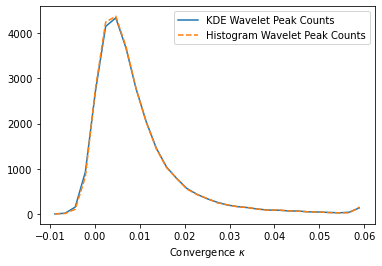
\includegraphics[width=\columnwidth]{figures/peakcounts.png}
    \caption{Comparison of traditional histogram-based peak counts, against our  KDE-based peak counts statistic. The two statistics are similar, but our KDE-based statistics is differentiable.}
    \label{fig:comp_statistics}
\end{figure}


\subsection{Wavelet $\ell_1$-norm}

\EiffL{Explain what's the deal with this l1 norm}




\section{Results}

\section{Discussion}

\subsection{Future directions}

\section{Conclusions}

%=====================
% END OF THE MAIN TEXT
%=====================

\end{document}
